\documentclass[10]{IEEEtran}

\usepackage{cite}
\usepackage{amsmath,amssymb,amsfonts}
\usepackage{algorithmic}
\usepackage{graphicx}
\usepackage{textcomp}
\def\BibTeX{{\rm B\kern-.05em{\sc i\kern-.025em b}\kern-.08em
		T\kern-.1667em\lower.7ex\hbox{E}\kern-.125emX}}

\begin{document}
	\title{Minimization of Cumulative Battery Aging: A Grid-Based Approach}
	\author{\IEEEauthorblockN{Yu-Hsin Huang}\textsuperscript{1},
		\and
	\IEEEauthorblockN{Yaser Marafee}\textsuperscript{1},
		\and
	\IEEEauthorblockN{Raja Selvakumar}\textsuperscript{1},
		\and
	\IEEEauthorblockN{Scott J. Moura}\textsuperscript{2} \\ \textsuperscript{1} \and \textit{Department of Chemistry, University of Berkeley, California} \\ \textsuperscript{2} \and \textit{Department of Civil Engineering, University of Berkeley, California} \\ \textbf{\texttt{\{yhh, yaser\_marafee, rselvak6, smoura\}@berkeley.edu}}
	}
	\maketitle
	\begin{abstract}
		Please disregard due to lack of experimental results for the progress report. All necessary discussions are handled in the summary.
	\end{abstract}
	
	\begin{IEEEkeywords}
		optimization and control, battery systems, aging
	\end{IEEEkeywords}

	\section{Introduction}
	
	\subsection{Motivation \& Background}
	Electrification of renewable energy integration and transportation of automobile compose two essential pathways towards the reduction of greenhouse gas emission and therefore the impact of global warming \cite{b1} The importance of energy storage devices can be seen in consumer electronics, electric vehicles, and grid storage. With increasing diversification in renewable and intermittent power supplies, larger integration of energy storage systems will be important. The main issue with batteries is aging during their lifetime due to the decrease in capacity, which leads to voltage decay and loss of power. There are numerous electrochemical mechanisms to describe aging \cite{b2, b3, b4}. However, characterization is challenging due to diverse time scales and complex nonlinearities in these models. Dynamic parameter estimation and battery state-of-charge (SOC) analysis remain complex topics.
	
	\begin{figure}[htbp]
		\centerline{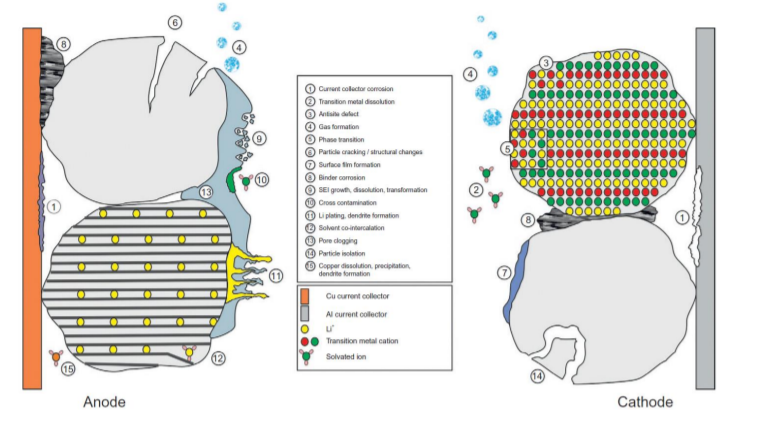
\includegraphics[keepaspectratio,height=0.5\textheight, width=0.5\textwidth]{fig1.png}}
		\caption{Examples of lithium ion battery aging mechanisms in EV applications.\cite{b4}}
		\label{f1}
	\end{figure}
	
	As Figure \ref{f1}demonstrates, there are a host of potential reasons for Li-ion aging. Current research has only been able to study capacity fade in smaller systems, and are limited to physical mathematical models without experimental insight.
	
	This project focuses on development of an optimization model which incorporates the grid storage and cell aging mechanisms. We try to investigate the capacity fade from parameters such as time, temperature, depth of discharge (DOD), and discharge rate as presented in Equation \ref{eq1}\cite{b5}:
	
	\begin{equation}\label{eq1}
	Q_{loss} = B\exp(\frac{-E_a}{RT})(A_h)^z
	\end{equation}
	where $Q_{loss}$ is the percentage of capacity loss, \textit{B} is the pre-exponential factor, $E_a$ is the activation energy in $\frac{J}{mol}$, \textit{R} is the gas constant, \textit{T} is the absolute temperature, and $A_h$ is the Ah-throughput, which is expressed as $A_h$ = (cycle number) $\cdot$ (DOD) $\cdot$ (full cell capacity), and \textit{z} is the power law factor. The work done by Wang et. al presents a relationship for the capacity fade from temperature and C-rate effects. For the purpose of this progress report, we will ignore these variations (as further indicated in the Assumptions section).
	
	Our group consists of three chemical engineering masters students in the Product Development Program. We have all taken classes in electrochemical systems, ranging from mathematical fundamentals to first steps of solid-electrolyte interphase (SEI) modelling. These experiences provide us an advantage to test the differences between black-box and white-box modelling approaches. As a team, our goal is to learn advanced control and parameter estimation techniques, so we hope to demonstrate this in our project results.
	
	\subsection{Relevant Literature}
	Battery cycling promotes capacity and power fade over time. We define capacity fade as the reduction in overall battery energy, while defining the power fade as the increase in resistance due to SEI formation or other bulk effects. As shown in Figure \ref{f2}A, cycling gradually damages the configuration of electrodes and therefore hinders the performance of the batteries, especially at high DOD. And as Figure \ref{f2}B shows, the increase in temperature causes an increase in degradation. Research has put emphasis on developing models to account for these mechanisms. 
	
	\begin{figure}[htbp]
		\centerline{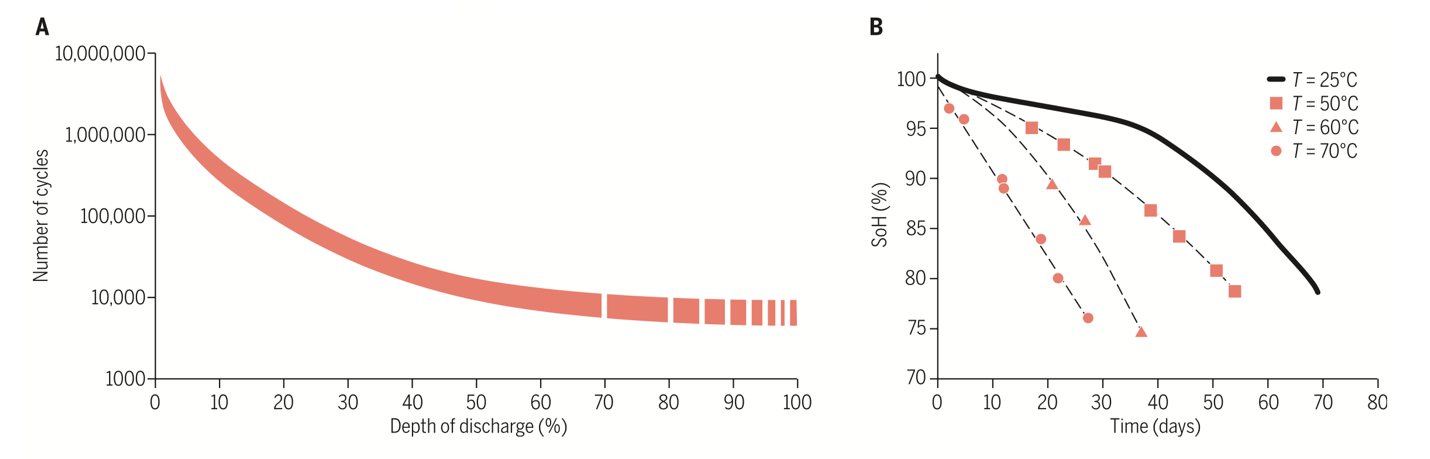
\includegraphics[keepaspectratio,height=0.5\textheight, width=0.5\textwidth]{fig3.png}}
		\caption{Influence of DoD and temperature on battery performance degradation. (A) Cycle life as a function of DOD for Li-ion cells operating at 25°C. (B) State of Health (SOH) as a function of time for Li-ion cells cycling at a rate of 1C at different temperatures.\cite{b1}}
		\label{f2}
	\end{figure}
	
	Battery aging can be classified into two main categories: calendar aging and cycle aging.\cite{b6} The former is associated with the phenomena and the consequences of battery storage and cycle aging corresponds to the influence of battery utilization time. Calendar aging is the irreversible process of lost capacity during storage. The battery is degraded due to self storage.  Temperature effects greatly contribute to calendar aging as side reactions are facilitated and cause capacity fade, as shown in figure \ref{f3}. The other principal variable under investigation in calendar aging is the State of Charge (SOC). The state of charge is equivalent to the ratio of the current battery energy to the maximum capacity. While operating at an increased SOC may result in greater energy throughput, this also results in larger capacity fade as indicated earlier in Equation \ref{eq1}.
	
	\begin{figure}[htbp]
		\centerline{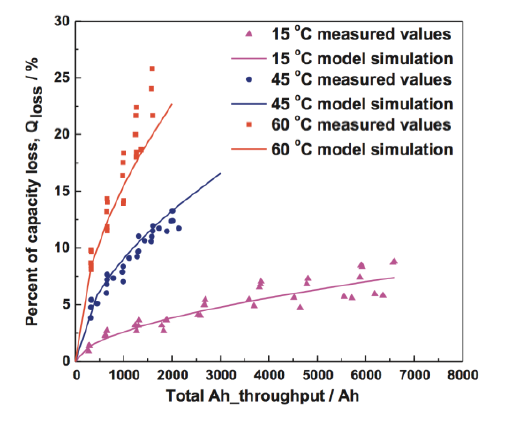
\includegraphics[keepaspectratio,height=0.5\textheight, width=0.5\textwidth]{fig4.png}}
		\caption{Simulation of cycle-life prediction for a LiFePO$_4$ at a C/2 discharge rate. \cite{b5}}
		\label{f3}
	\end{figure}
	
	Cycle aging originates from charging or discharging of the battery. Many factors are involved with this kind of aging- including the above mentioned factors for calendar aging. Charging/discharging voltages also impact the battery aging and should be taken into consideration. Two principal changes are observed in a cell as it degrades: it loses capacity and its impedance increases. As shown in Figure \ref{f4}, they can be classified into three types: electrochemical models, performance-based models, and equivalent-circuit-based models.
	
	\begin{figure}[htbp]
		\centerline{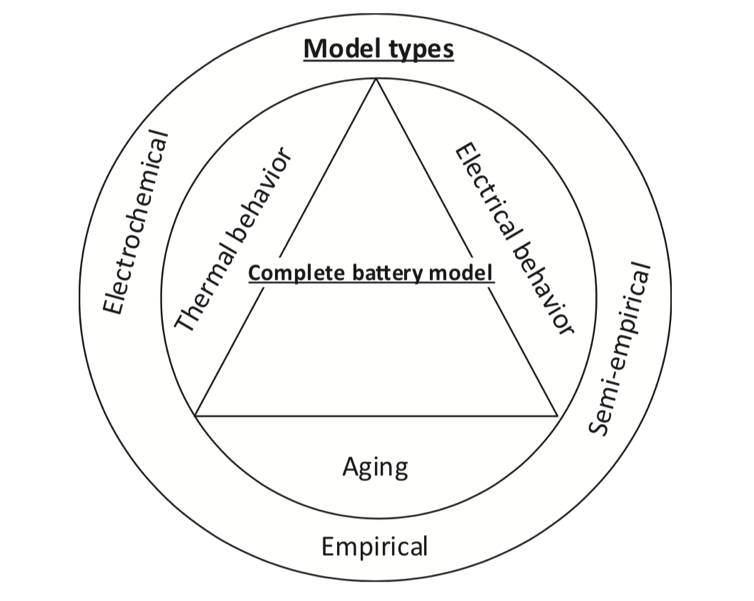
\includegraphics[keepaspectratio,height=0.3\textheight, width=0.3\textwidth]{fig5.png}}
		\caption{Different battery modelling schemes. \cite{b7}}
		\label{f4}
	\end{figure}

	\subsection{Focus of this Study}
	This study will focus on studying capacity fade in distributed rechargeable battery technologies by intimation the battery fleet with grid distribution system. We break down our focus into two parts: a) understanding parameters such as temperature, SOC, SOH, and DOD that contribute to battery aging and material degradation and b) designing a control framework to optimally distribute power to/from the battery fleet. With this two-prong focus we aim to automate battery monitoring, hopefully even when faced with unpredictable thermal and catalytic degradation.
	
	\section{Technical Description}
	\subsection{Assumptions}
	We first itemize the assumptions we have made for the first progress report. We hope to expand on some of these assumptions over the course of the semester:
	
	\begin{itemize}
		\item Power can flow freely between nodes (as we will define below) while neglecting heat losses and line capacity
		\item Power can be drawn from the main power source, and we assume it has a maximum capacity $C_{max}$ over all time \textit{T}
		\item Power flow from the source is unidirectional (i.e. we only consider charging)
		\item Power flow between nodes is bidirectional
		\item The node represents a power distribution center, where the balance from power demanded and power transmitted is the power storage
		\item Each node is responsible for its own localized power demand
		\item Battery temperature is constant with ambient conditions
		\item Power throughput is controlled at a constant C-rate\footnote{This is based on the relationship between power and energy as: $\frac{P}{E}$ = C-rate}
		\item Grid batteries used are Li-ion
	\end{itemize}
	\subsection{Formulation}
	We now define our grid and the appropriate parameters. For the purposes of this progress report, we show a sample grid in Figure \ref{f5}. Table \ref{t1} includes all the definitions for the variables and parameters used in this formulation.
	
	The objective function is to minimize the cumulative aging across all nodes $j\in[1,J]$, as shown in Equation \ref{eq2}. Note that \textit{J} represents the total nodes in the grid space.
	\begin{equation}\label{eq2}
	min\sum_{j\in J}^{}Q_{loss,j} = min\sum_{k\in T}^{}\sum_{j\in J}^{}\beta(A_{h,j}[k])^z
	\end{equation}
	Discretization of the problem allows for a simple reference formulation to characterize the complex electrochemical reactions. This optimization problem is subject to the following constraints:
	\begin{equation}\label{eq3}
	p_j[k] = \sum_{i\in J}^{}A_{ij}P_{ji}[k]-\sum_{j\in J}^{}A_{ji}P_{ij}[k]-d_j[k]
	\end{equation}
	\begin{equation}\label{eq4}
	E_j[k+1] = E_j[k] + p_j[k]\cdot\Delta t \quad \forall j\in J, k\in T
	\end{equation}
	\begin{equation}\label{eq5}
	\sum_{j\in J}^{}P_{0j} \leq C_{max}
	\end{equation}
	\begin{equation}\label{eq6}
	P_{ij} \geq 0 \quad \forall i,j\in J
	\end{equation}
	\begin{equation}\label{eq7}
	E_{min} \leq E_j[k] \leq E_{max} \quad \forall j\in J, k\in T
	\end{equation}
	\begin{equation}\label{eq8}
	d_j[k] \geq 0 \quad \forall j\in J, k\in T
	\end{equation}
	\begin{equation}\label{eq9}
	P_{ji}[k] = 0 \quad \forall j\in J, i=0
	\end{equation}
	Equation \ref{eq3} represents the power balance at time \textit{k}. The sign of $p_j$ determines whether the battery will be charged or discharged at this point. Equation \ref{eq4} is the discretized integrator expression for energy. Equation \ref{eq5}-\ref{eq8} represent the limits on the power transmitted from the source, power transmitted between nodes, the energy states, and the demand respectively. Equation \ref{eq9} indicates our earlier assumption that power can only be received from the source, not returned if there is a demand shortage.
	For $z\leq 0.5$, this problem is convex.  
	
	\begin{table}[htbp]
		\caption{List of parameters and variables used in formulation}
		\begin{center}
			\begin{tabular}{l|l|l}
				\hline 
				\textbf{Symbol}&\textbf{Description}&\textbf{Units} \\ \hline
				$Q_{loss,j}$ & Capacity loss of node \textit{j} & [W-h]\\
				$\beta$ & Pre-exponential factor$^{\mathrm{a}}$ & [-]\\
				$A_h$ & Amp hour throughput & [C]\\ 
				$z$ & Power law factor & [-] \\ \hline
				$A$ & Adjacency matrix encoding network structure & [-]\\
				$p_j$ & Power charged or discharged at node \textit{j} & [W]\\
				$d_j$ & Power demand at node \textit{j} & [W]\\
				$P_{ij}$ & Power delivered from node \textit{i} to node \textit{j} & [W]\\
				$E_j[k]$ & Energy available to the node \textit{j} at time \textit{k} & [W-h]\\ \hline
				$C_{max}$ & Maximum capacity available from the source & [W]\\
				$\Delta T$ & Simulation time step & [h]\\
				$T$ & Total simulation time & [h]\\
				$E_{min}$,$E_{max}$ & Minimum and maximum energy limits$^{\mathrm{b}}$ & [W-h]\\
			\hline
			\multicolumn{3}{l}{$^{\mathrm{a}}$Currently constant, will change with temperature variance}\\
			\multicolumn{3}{l}{$^{\mathrm{b}}$This is derived from the C-rate.}	
			\end{tabular}
			\label{t1}
		\end{center}
	\end{table}
	
	\begin{figure}[htbp]
		\centerline{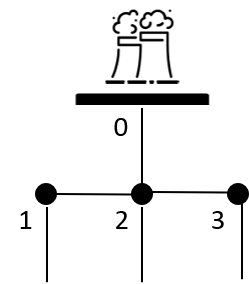
\includegraphics{fig6.png}}
		\caption{Trial 3 node battery storage grid.}
		\label{f5}
	\end{figure}
	
	\section{Discussion}
	Please disregard due to lack of experimental results for the progress report. All necessary discussions are handled in the summary.
	
	\section{Summary}
	We have studied the formulation of cumulative aging in distributed battery networks. We use a network based approach to model the power delivery between different energy systems. Through the current progress report we present our first attempt at a problem formulation. Over the course of the semester, we hope to (1) further analyze the $A_h$ term for different C-rates and depths of discharge (DOD) (2) introduce uncontrollable temperature fluctuations to observe system capacity loss (3) test the equations with real data and conduct sensitivity analysis on the initial charge states $E_j[0] \; \forall j\in J$ (4) attempt to model the capacity at each time point $k$ using an Extended Kalman Filter\cite{b8} and (5) introduce intermittency in the power source to model the impact of solar PV in the grid system. We are excited about our groundwork in the first half of the semester and look forward to stretching our knowledge of the subject material in the second half.
	
	\section*{Acknowledgment}
	The authors would like to thank the University of California, Berkeley and Scott Moura, in particular, for the support and insight behind this project. The authors are also grateful to the groundwork set forth by the previous CE 295 team to create a framework for understanding battery aging.
	
	\begin{thebibliography}{00}
		\bibitem{b1} Palacin, M. R.; de Guibert, A., ''Why do batteries fail?'' Science 2016, 351 (6273), 7.
		\bibitem{b2} Baek, K.W., Hong, E.S. \& Cha, S.W. Int. J Automot. Technol. (2015) 16: 309. https://doi.org/10.1007/s12239-015-0033-2
		\bibitem{b3} Pinson, M. B., Bazant, M. Z (2013). ''Theory of SEI Formation in Rechargeable Batteries: Capacity Fade, Accelerated Aging and Lifetime Prediction.'' Journal of The Electrochemical Society. Volume 160. Pages A243-A250. 
		\bibitem{b4} Vetter, J.; Novak, P.; Wagner, M. R.; Veit, C.; Moller, K. C.; Besenhard, J. O.; Winter, M.; Wohlfahrt-Mehrens, M.; Vogler, C.; Hammouche, A., ''Ageing mechanisms in lithium-ion batteries.'' J. Power Sources 2005, 147 (1-2), 269-281.
		\bibitem{b5} Wang, J.; Liu, P.; Hicks-Garner, J.; Sherman, E.; Soukiazian, S.; Verbrugge, M.; Tataria, H.; Musser, J.; Finamore, P., ''Cycle-life model for graphite-LiFePO4 cells.'' J. Power Sources 2011, 196 (8), 3942-3948.
		\bibitem{b6} Barre, A.; Deguilhem, B.; Grolleau, S.; Gerard, M.; Suard, F.; Riu, D., ''A review on lithium-ion battery ageing mechanisms and estimations for automotive applications.'' J. Power Sources 2013, 241, 680-689.
		\bibitem{b7} Jaguemont, J.; Boulon, L.; Dube, Y., ''A comprehensive review of lithium-ion batteries used in hybrid and electric vehicles at cold temperatures.'' Applied Energy 2016, 164, 99-114.
		\bibitem{b8} Plett, G. L., ''Extended Kalman filtering for battery management systems of LiPB-based HEV battery packs.'' Journal of Power Sources 2004, 134, 262-276
	\end{thebibliography}
	
\end{document}